\chapter{Hallway Usability Testing}

\section{Survey setup}
\begin{flushleft}


The participants were given a mobile phone with the preinstalled app. Several Bluetooth devices were already paired with the phone. They were also handed a printed questionnaire.

The only initial information given was the introduction part of the questionnaire. The participants were encouraged to explore and comment. If they got stuck on a part for a longer time they were offered a clue how to proceed. If they had questions they were generally answered.

After they were done exploring they filled out the questionnaire.

The interactions were observed by a team member, to ensure a good experience and to find out how the users interacted with the app.

The survey was conducted at a university event. Most of the participants are students and graduates.

There were 9 Participants.

\section{Questionnaire}
Please see the following two pages.
\newpage
\includepdf[pages=-]{tex/survey}
\section{Results}
\subsection{Questionnaire evaluation}

\resizebox {\textwidth/2} {!} {
	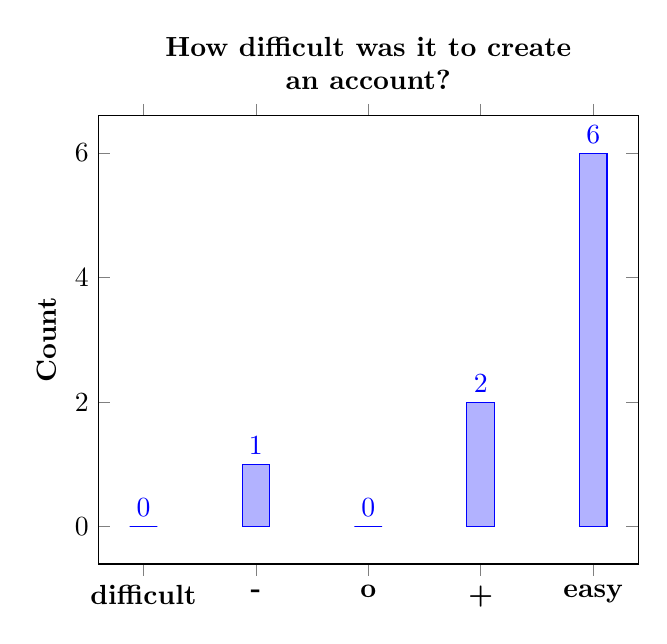
\begin{tikzpicture}
	\begin{axis}[
		title={How difficult was it to create \\ an account?},
		align = center,
		font=\bfseries,
		ybar,
		ylabel=Count,
		symbolic x coords={difficult, -, o, +, easy},
		nodes near coords, 
		nodes near coords align={vertical},
	]
	\addplot coordinates {(difficult,0) (-,1) (o,0) (+,2) (easy,6)};
	\end{axis}
	\end{tikzpicture}
}\resizebox {\textwidth/2} {!} {
	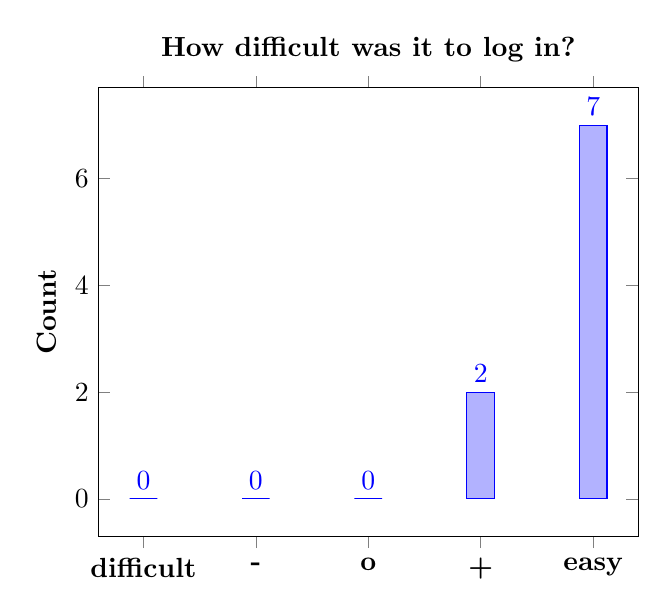
\begin{tikzpicture}
	\begin{axis}[
	title=How difficult was it to log in?,
	align = center,
	font=\bfseries,
	ybar,
	ylabel=Count,
	symbolic x coords={difficult, -, o, +, easy},
	nodes near coords, 
	nodes near coords align={vertical},
	]
	\addplot coordinates {(difficult,0) (-,0) (o,0) (+,2) (easy,7)};
	\end{axis}
	\end{tikzpicture}
}

\resizebox {\textwidth/2} {!} {
	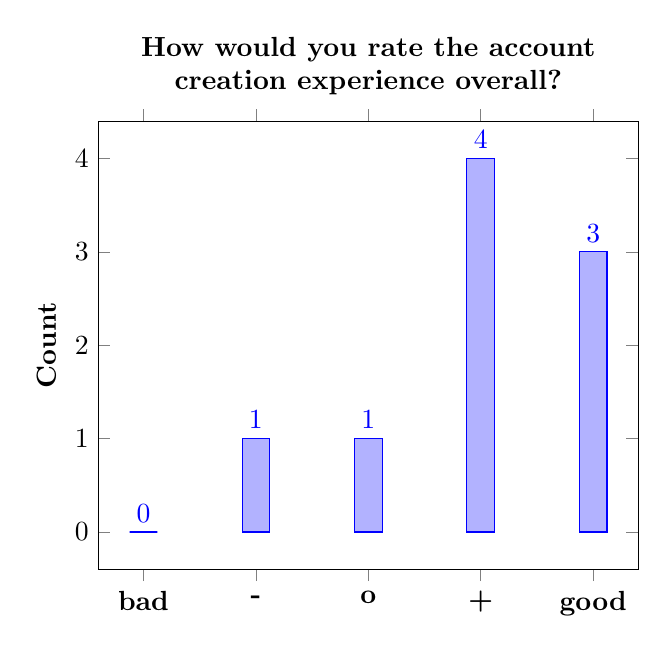
\begin{tikzpicture}
	\begin{axis}[
	title={How would you rate the account \\ creation experience overall?},
	align = center,
	font=\bfseries,
	ybar,
	ylabel=Count,
	symbolic x coords={bad, -, o, +, good},
	nodes near coords, 
	nodes near coords align={vertical},
	]
	\addplot coordinates {(bad,0) (-,1) (o,1) (+,4) (good,3)};
	\end{axis}
	\end{tikzpicture}
}

\textbf{Do you have any comments or suggestions for account creation and login?}
\begin{itemize}
	\item Password guideline missing
	\item User verification (password)
	\item Errors werfen
	\item Unerwartete Frage beim Account erstellen und keine Info, dass Anklicken erforderlich ist zur Accounterstellung
	\item auto-login after creating an account
	\item Rückmeldung, dass ein Account erfolgreich erstellt wurde Er jetzt verwendet werden kann
	\item No warnings (missing name), No errors (server not reachable)
	\item No existing user check: Register as "baum" was "successful" (but did not create account), leaving all fields except "sell soul" registers "successful" (redirect to login)
\end{itemize}

\resizebox {\textwidth/2} {!} {
	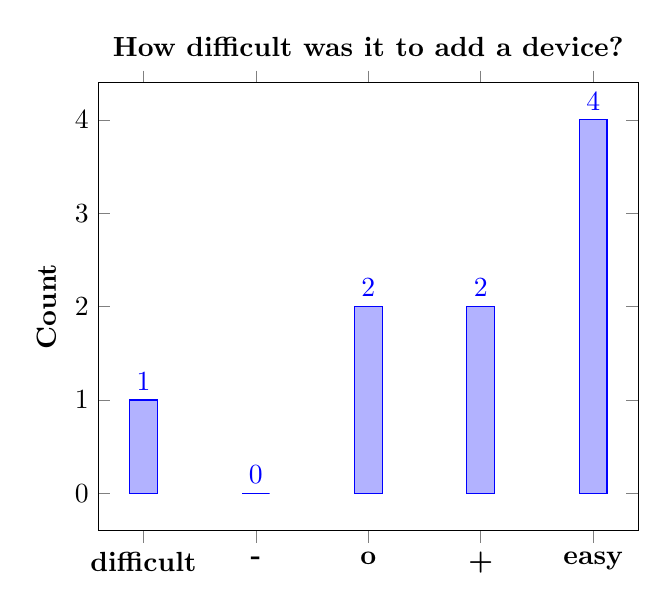
\begin{tikzpicture}
	\begin{axis}[
	title={How difficult was it to add a device?},
	align = center,
	font=\bfseries,
	ybar,
	ylabel=Count,
	symbolic x coords={difficult, -, o, +, easy},
	nodes near coords, 
	nodes near coords align={vertical},
	xtick=data,
	]
	\addplot coordinates {(difficult,1) (-,0) (o,2) (+,2) (easy,4)};
	\end{axis}
	\end{tikzpicture}
}\resizebox {\textwidth/2} {!} {
	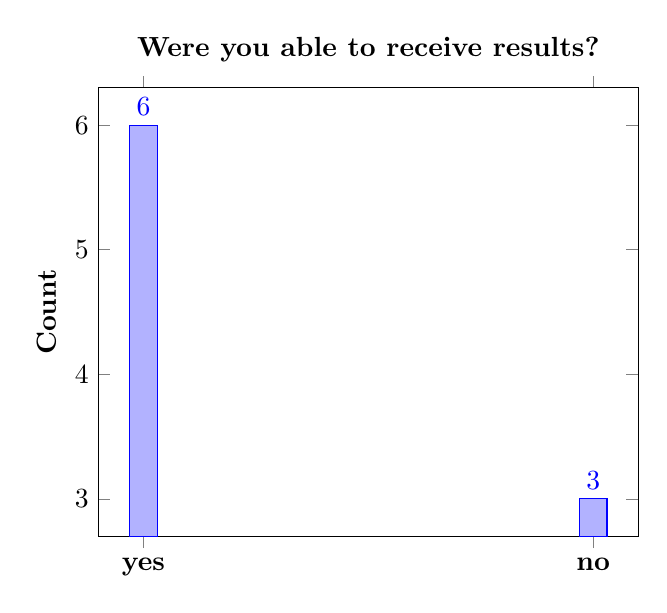
\begin{tikzpicture}
	\begin{axis}[
	title={Were you able to receive results?},
	align = center,
	font=\bfseries,
	ybar,
	ylabel=Count,
	symbolic x coords={yes, no},
	nodes near coords, 
	nodes near coords align={vertical},
	xtick=data,
	]
	\addplot coordinates {(no,3) (yes,6)};
	\end{axis}
	\end{tikzpicture}
}

\resizebox {\textwidth/2} {!} {
	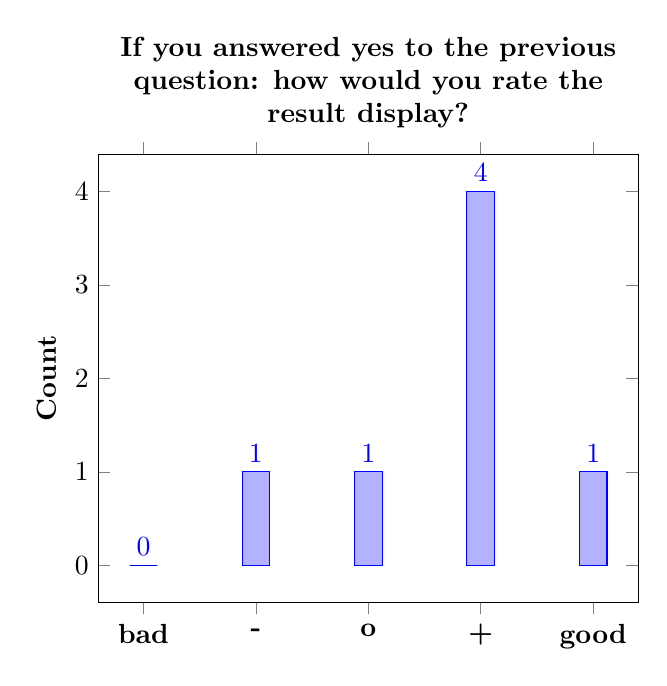
\begin{tikzpicture}
	\begin{axis}[
	title={If you answered yes to the previous \\ question: how would you rate the \\ result display?},
	align = center,
	font=\bfseries,
	ybar,
	ylabel=Count,
	symbolic x coords={bad, -, o, +, good},
	nodes near coords, 
	nodes near coords align={vertical},
	]
	\addplot coordinates {(bad,0) (-,1) (o,1) (+,4) (good,1)};
	\end{axis}
	\end{tikzpicture}
}

\textbf{Do you have any comments or suggestions for the device management functionality?}
\begin{itemize}
	\item Die Ansicht mit den Geräten war von der Ansicht, wo man ein Gerät hinzufügt optisch schwer zu unterscheiden, ich war kurz verwirrt
	\item make device-type editable
	\item Beim "Account löschen keine Info, dass der Account gelöscht wurde
	\item local time
	\item copyright (osm)
	\item Trace (gps)
	\item "Map provider" (incompatible to) List view
	\item not obvious that devices have to be paired first in android
	\item enable bluetooth (warning[preferred] or auto [but on leave redisable] - best as setting) as no paired devices will be shown without
\end{itemize}

\resizebox {\textwidth/2} {!} {
	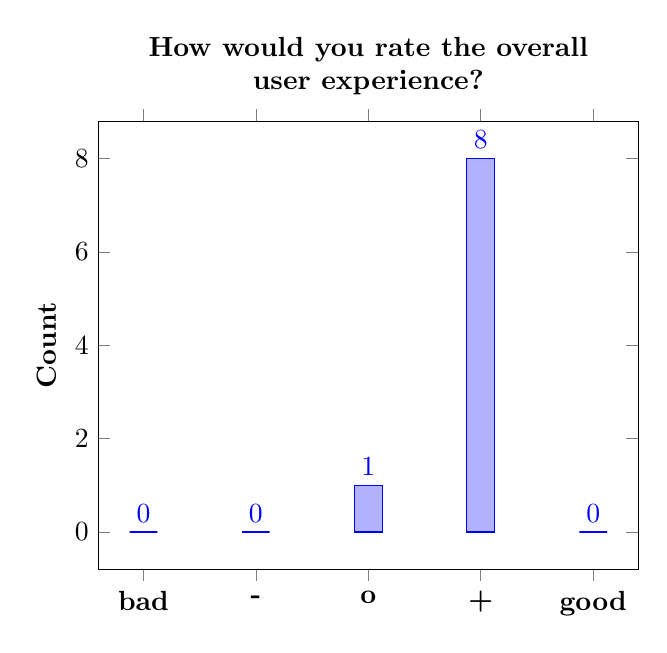
\begin{tikzpicture}
	\begin{axis}[
	title={How would you rate the overall \\ user experience?},
	align = center,
	font=\bfseries,
	ybar,
	ylabel=Count,
	symbolic x coords={bad, -, o, +, good},
	nodes near coords, 
	nodes near coords align={vertical},
	]
	\addplot coordinates {(bad,0) (-,0) (o,1) (+,8) (good,0)};
	\end{axis}
	\end{tikzpicture}
}\resizebox {\textwidth/2} {!} {
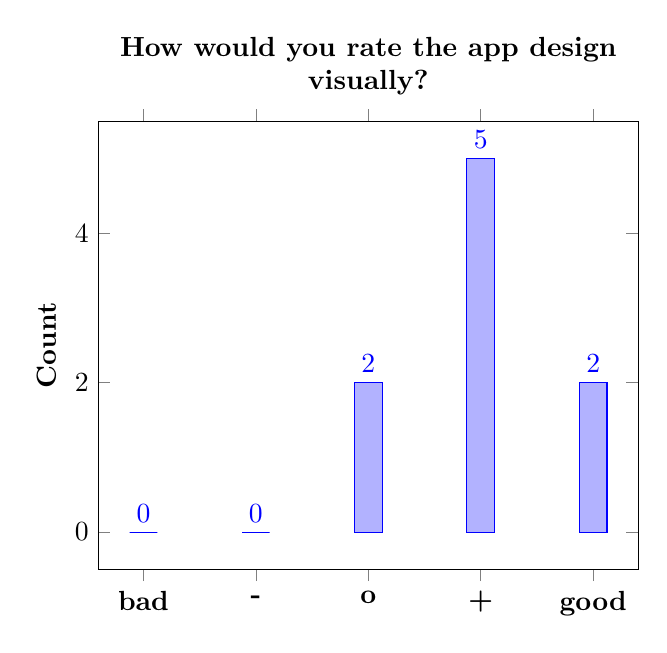
\begin{tikzpicture}
	\begin{axis}[
	title={How would you rate the app design \\ visually?},
	align = center,
	font=\bfseries,
	ybar,
	ylabel=Count,
	symbolic x coords={bad, -, o, +, good},
	nodes near coords, 
	nodes near coords align={vertical},
	]
	\addplot coordinates {(bad,0) (-,0) (o,2) (+,5) (good,2)};
	\end{axis}
	\end{tikzpicture}
}

\resizebox {\textwidth/2} {!} {
	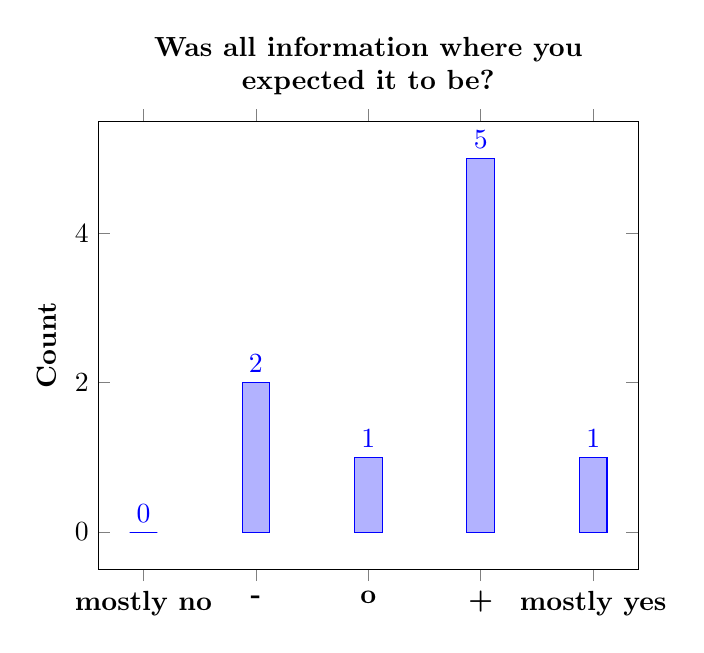
\begin{tikzpicture}
	\begin{axis}[
	title={Was all information where you \\ expected it to be?},
	align = center,
	font=\bfseries,
	ybar,
	ylabel=Count,
	symbolic x coords={mostly no, -, o, +, mostly yes},
	nodes near coords, 
	nodes near coords align={vertical},
	]
	\addplot coordinates {(mostly no,0) (-,2) (o,1) (+,5) (mostly yes,1)};
	\end{axis}
	\end{tikzpicture}
}\resizebox {\textwidth/2} {!} {
	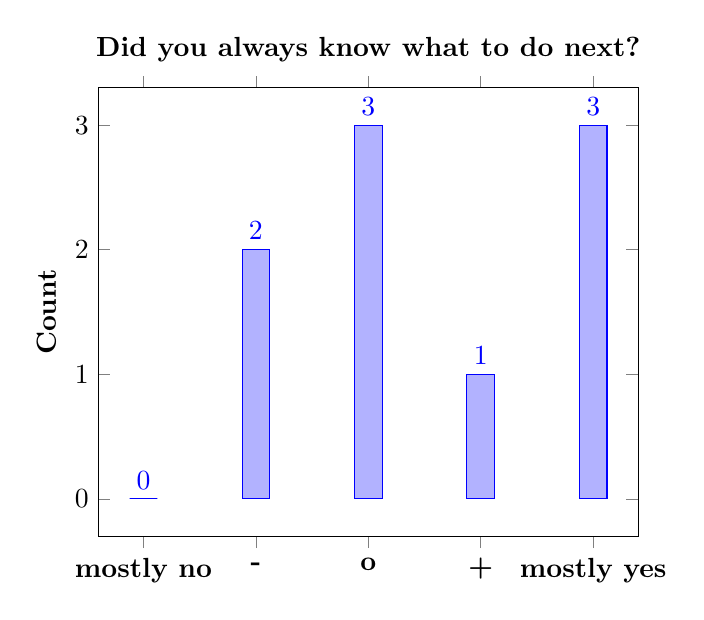
\begin{tikzpicture}
	\begin{axis}[
	title={Did you always know what to do next?},
	align = center,
	font=\bfseries,
	ybar,
	ylabel=Count,
	symbolic x coords={mostly no, -, o, +, mostly yes},
	nodes near coords, 
	nodes near coords align={vertical},
	]
	\addplot coordinates {(mostly no,0) (-,2) (o,3) (+,1) (mostly yes,3)};
	\end{axis}
	\end{tikzpicture}
}

\resizebox {\textwidth/2} {!} {
	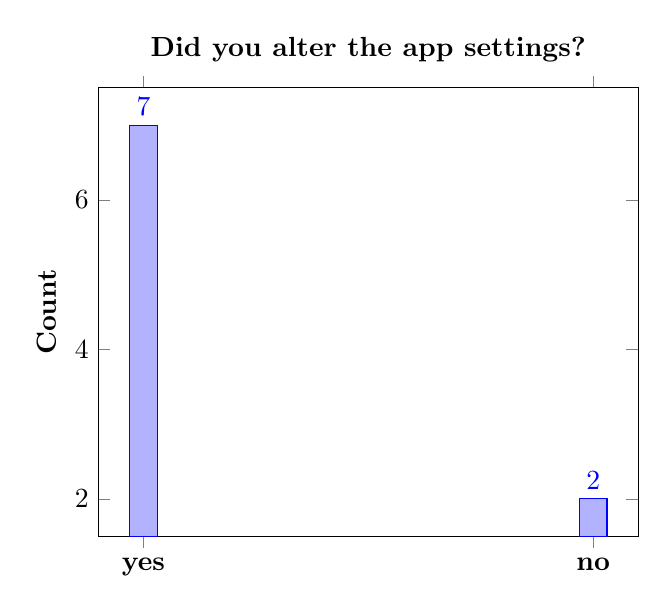
\begin{tikzpicture}
	\begin{axis}[
	title={Did you alter the app settings?},
	align = center,
	font=\bfseries,
	ybar,
	ylabel=Count,
	symbolic x coords={yes, no},
	nodes near coords, 
	nodes near coords align={vertical},
	xtick=data,
	]
	\addplot coordinates {(no,2) (yes,7)};
	\end{axis}
	\end{tikzpicture}
}\resizebox {\textwidth/2} {!} {
	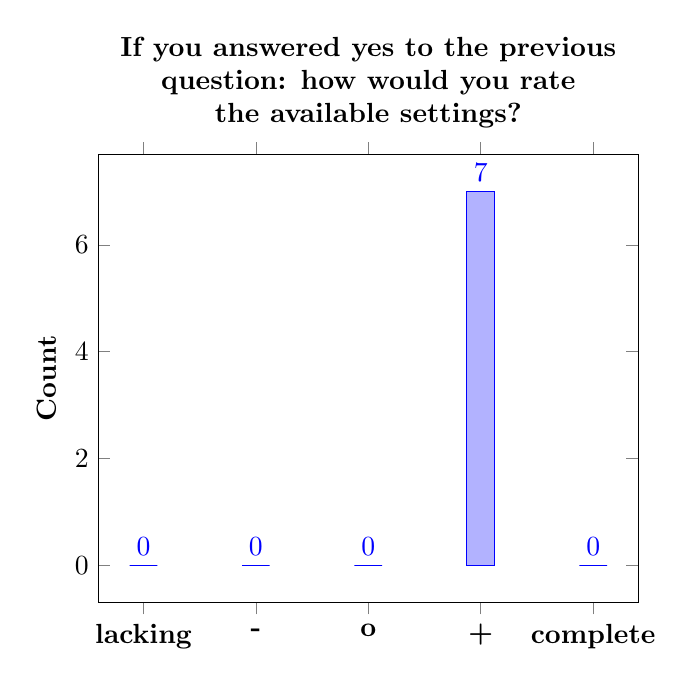
\begin{tikzpicture}
	\begin{axis}[
	title={If you answered yes to the previous \\ question: how would you rate \\ the available settings?},
	align = center,
	font=\bfseries,
	ybar,
	ylabel=Count,
	symbolic x coords={lacking, -, o, +, complete},
	nodes near coords, 
	nodes near coords align={vertical},
	]
	\addplot coordinates {(lacking,0) (-,0) (o,0) (+,7) (complete,0)};
	\end{axis}
	\end{tikzpicture}
}



\textbf{Which parts, screens or functionalities gave you any trouble or were difficult to use?}
\begin{itemize}
	\item Wechsel zwischen Kartenansicht und Liste (Liste vielleicht immer und bei Klicken auf einen Wert wechselt man auf die Karte)
	\item Delete schwer als button zu identifizieren
	\item Wirkt unausgereift, fehlende Fehlermeldung
	\item "Add Device"
	\item Add Device without bluetooth enabled
\end{itemize}
\par

\textbf{What did you like about this app?}
\begin{itemize}
	\item clear and simple, single purpose functionality
	\item Cleane Android Umgebung, wenig Ablenkung führt zu klarer Bedienbarkeit
	\item The map shows many details
	\item Einfach und funktional, klarer Aufbau, kein komplizierter Aufbau
	\item slick (less is more)
\end{itemize}

\par

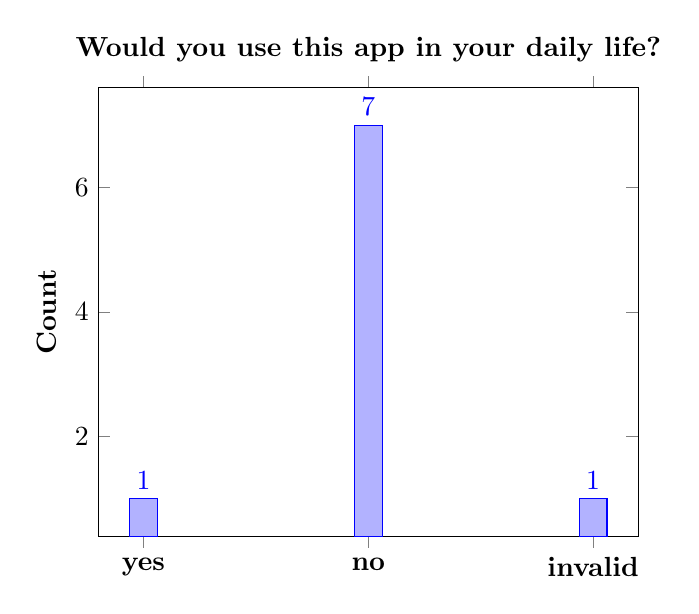
\begin{tikzpicture}
\begin{axis}[
title={ Would you use this app in your daily life?},
align = center,
font=\bfseries,
ybar,
ylabel=Count,
symbolic x coords={yes, no, invalid},
nodes near coords, 
nodes near coords align={vertical},
xtick=data,
]
\addplot coordinates {(no,7) (yes,1) (invalid, 1)};
\end{axis}
\end{tikzpicture}

\textbf{If you answered no to the previous question: Why not?}
\begin{itemize}
	\item Nutze selten Bluetooth Geräte
	\item Ist doch praktisch. Vielleicht Bedenken, was mit den gesammelten Daten passiert
	\item Benutze zu wenige BT-Devices, damit sich das lohnen würde
	\item I think I have no use for it
	\item too few bluetooth devices to track
	\item nicht ausgereift
	\item data protection / no devices
	\item not using bluetooth permanently due to battery concerns
	\item Too few bluetooth devices, but with more or after loosing some, yes
	
\end{itemize}

\textbf{Additional comments:}
\begin{itemize}
	\item DSGVO?
	\item Info Page (about this app, licences, authors...)
\end{itemize}

\end{flushleft}
